\documentclass[tikz,border=10pt]{standalone}
\usetikzlibrary{shapes.geometric, arrows.meta, positioning}

\tikzset{
    block/.style = {rectangle, draw, fill=blue!20, text width=5em, text centered, rounded corners, minimum height=4em},
    line/.style = {draw, thick, -Stealth},
    decision/.style={diamond, draw, fill=green!20, text width=5em, text badly centered, node distance=3cm, inner sep=0}
}

\begin{document}
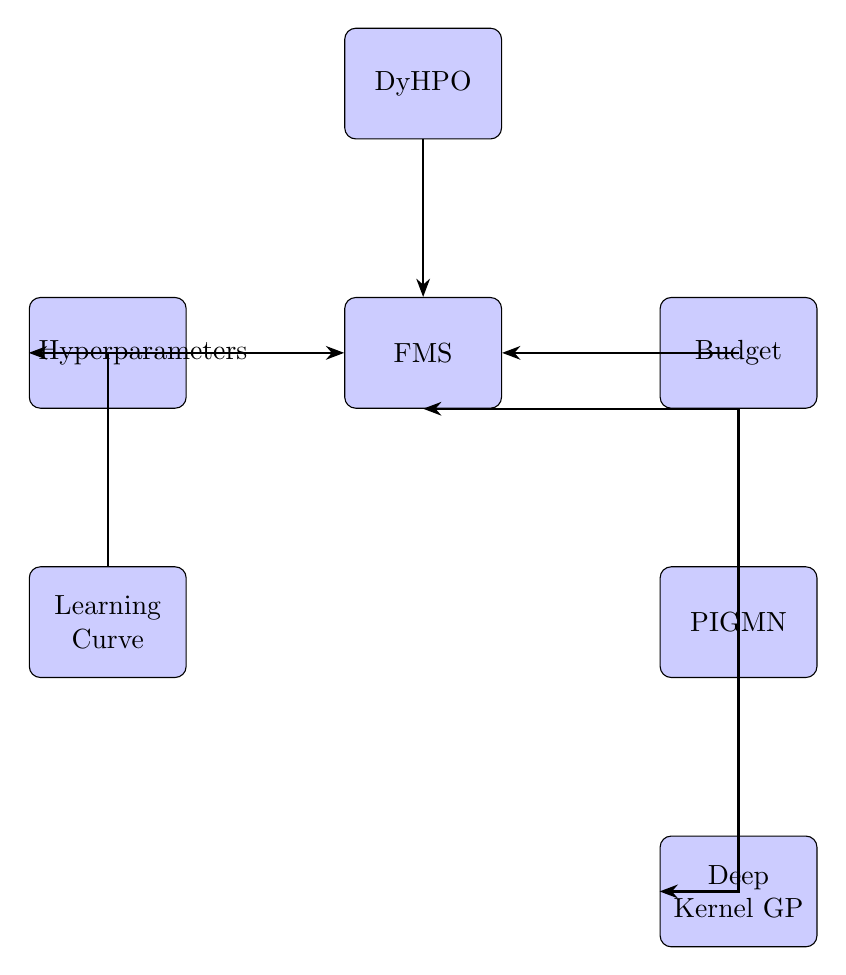
\begin{tikzpicture}[node distance=2cm]
    % Nodes
    \node (dyhpo) [block] {DyHPO};
    \node (fms) [block, below=of dyhpo] {FMS};
    \node (hyperparameters) [block, left=of fms] {Hyperparameters};
    \node (budget) [block, right=of fms] {Budget};
    \node (learning_curve) [block, below=of hyperparameters] {Learning Curve};
    \node (pigmn) [block, below=of budget] {PIGMN};
    \node (dkgp) [block, below=of pigmn] {Deep Kernel GP};

    % Lines
    \path [line] (dyhpo) -- (fms);
    \path [line] (hyperparameters) |- (fms.west);
    \path [line] (budget) |- (fms.east);
    \path [line] (learning_curve) |- (hyperparameters.west);
    \path [line] (pigmn) |- (dkgp.west);
    \path [line] (dkgp) |- (fms.south);
\end{tikzpicture}
\end{document}